% !TEX root = WWW.tex
\begin{figure*}[!ht]
\centering
\subfloat[\small Fat and thin vertices vs. threshold values]{
    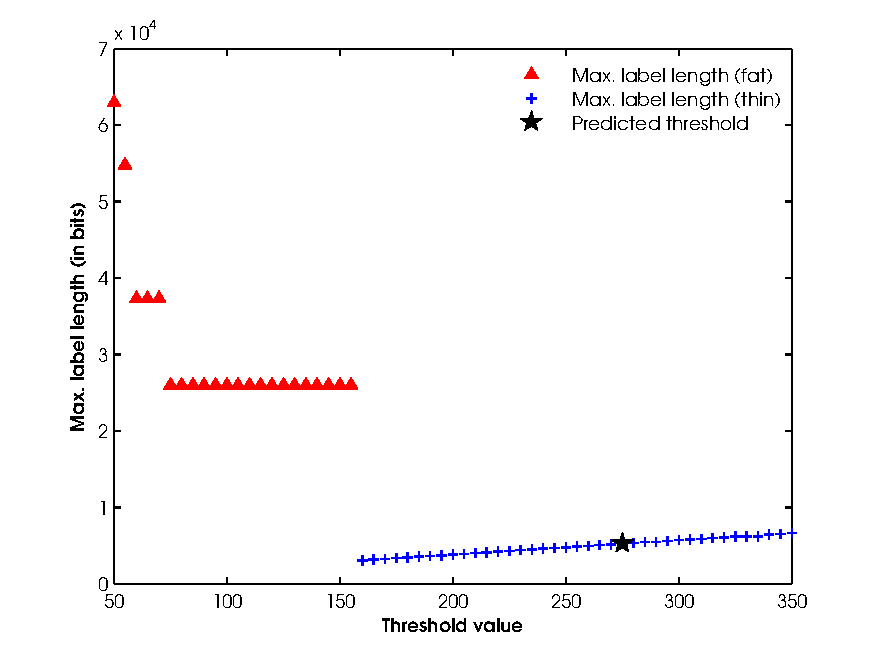
\includegraphics[width=0.4\textwidth]{Figures/barabasi-www.pdf}
}
\subfloat[\small Power law fit]{
    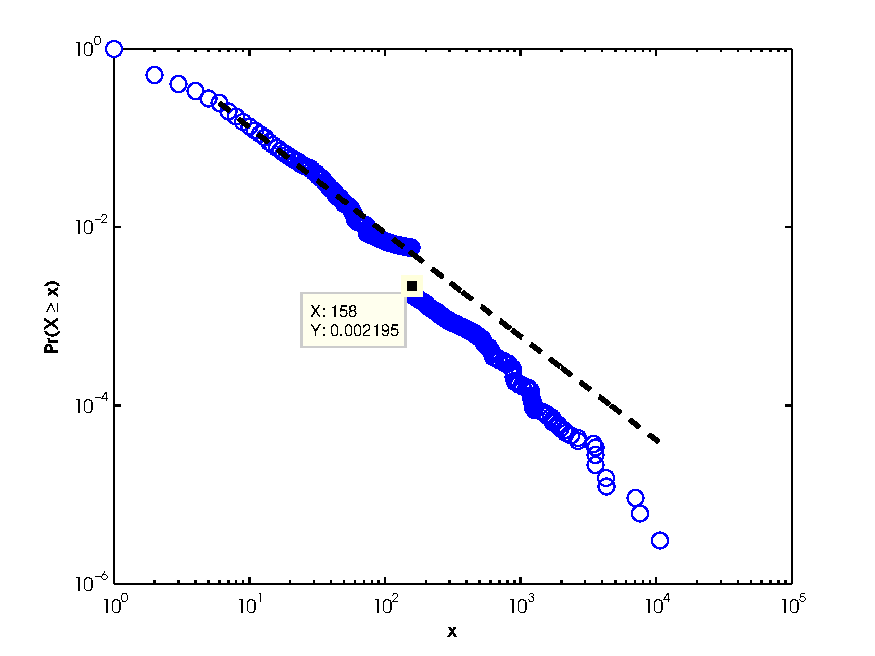
\includegraphics[width=0.4\textwidth]{Figures/barabasi-www-ccdf.pdf}
}%
\quad
\subfloat[\small Fat and thin vertices vs. threshold values]{
    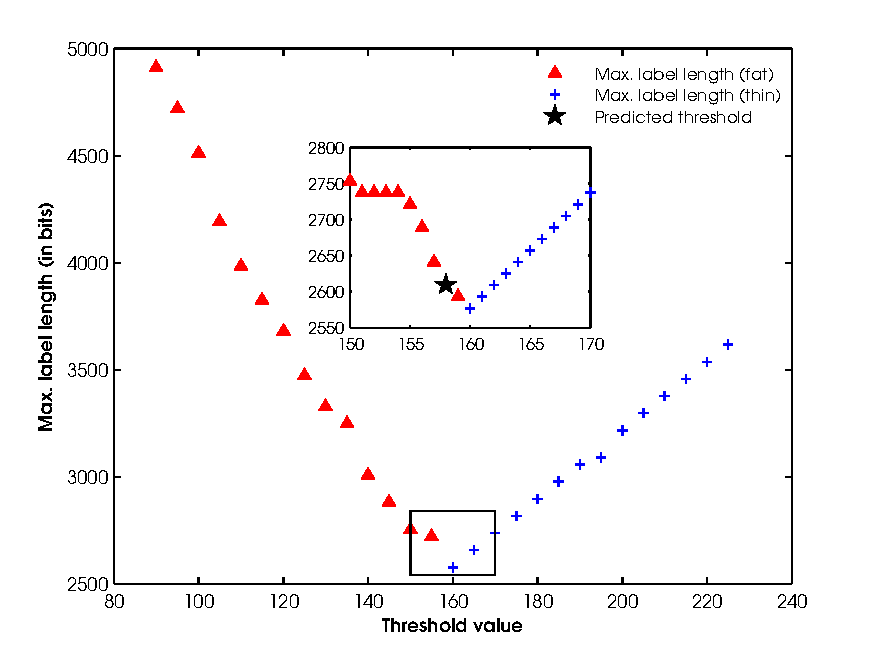
\includegraphics[width=0.4\textwidth]{Figures/enron-mail.pdf}
}
\subfloat[\small Power law fit]{
    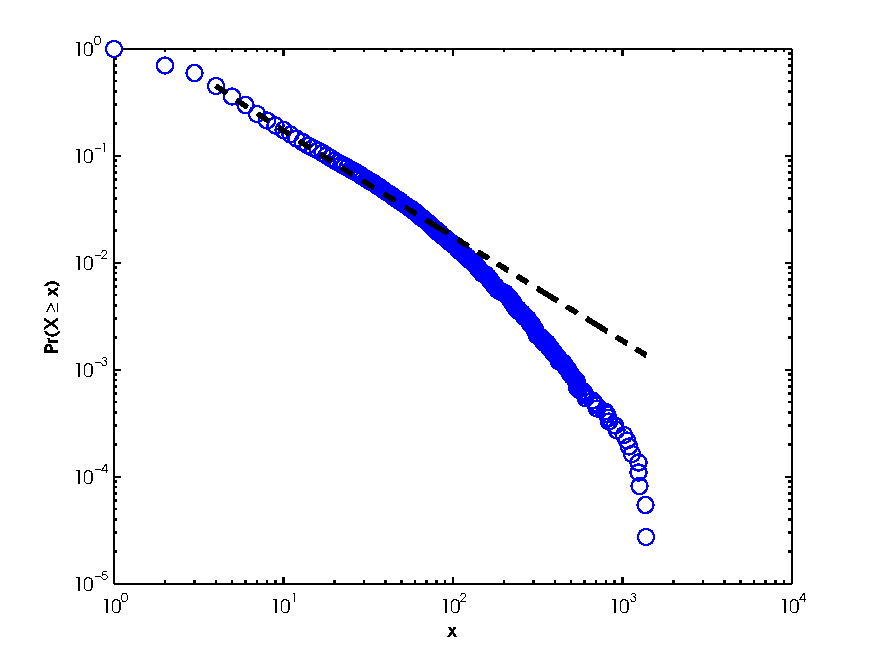
\includegraphics[width=0.4\textwidth]{Figures/enron-mail-ccdf.pdf} 
}%
\quad
\subfloat[\small Fat and thin vertices vs. threshold values]{
    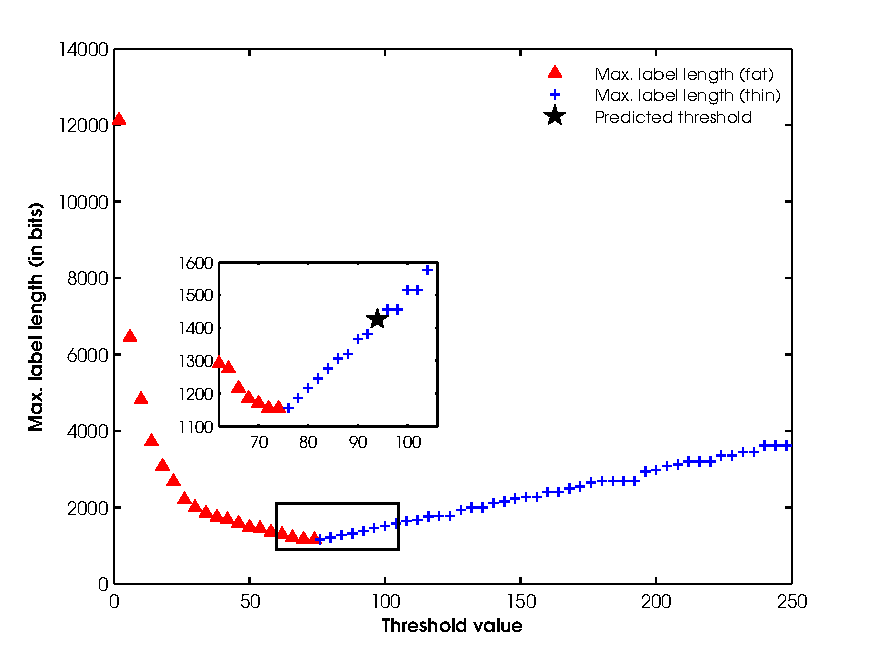
\includegraphics[width=0.4\textwidth]{Figures/internet.pdf}
}
\subfloat[\small Power law fit]{
    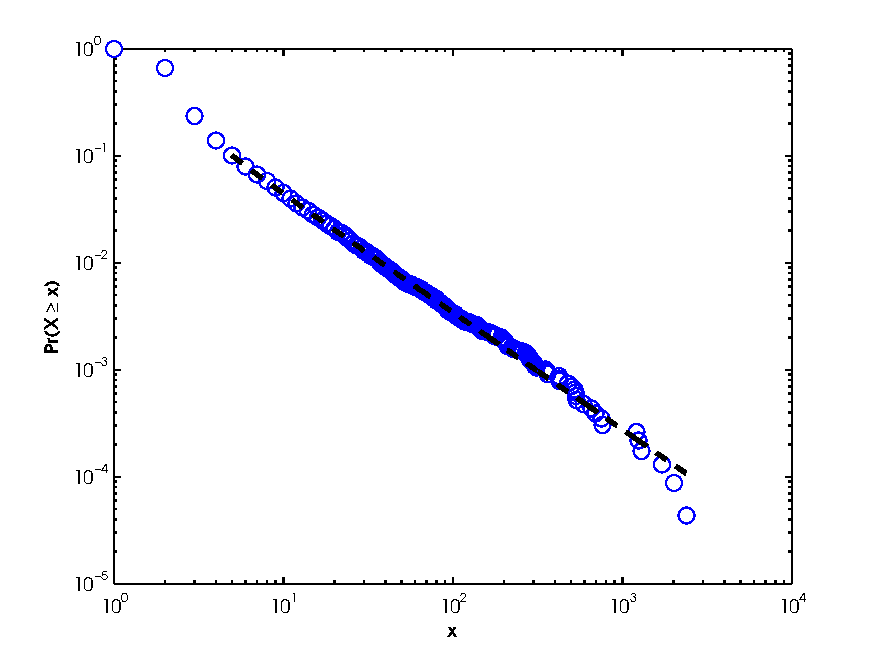
\includegraphics[width=0.4\textwidth]{Figures/internet-ccdf.pdf}
}%
\caption{Left: Fat and thin vertices plotted against increasing threshold values for the \textsc{enron} email communication dataset. The black pentagram is the predicted threshold ($1/\zeta(\alpha)\sqrt[\alpha](n)$) rounded to the nearest integer.  Right: Best-fitting power law ($\alpha = 1.97$)  superimposed on the complementary cumulative distribution function (CCDF) using the framework by \cite{clauset2009power}.}%
\label{fig:synthetic300}%
\end{figure*}